\documentclass[tikz]{standalone}
\usetikzlibrary{arrows}
\begin{document}
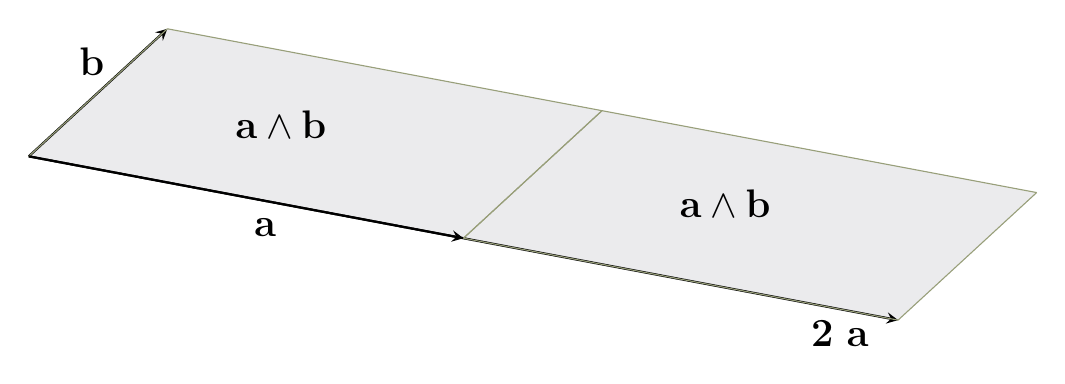
\begin{tikzpicture}[scale=1.0]

% ------------------------------------------------ lin_alg theme colors
\definecolor{la_white}{RGB}{233,235,223} %#E9EBDF
\definecolor{la_dark}{RGB}{59,54,81}     %#3B3651
\definecolor{la_gray}{RGB}{96,112,139}   %#60708B
\definecolor{la_tan}{RGB}{152,159,122}   %#989F7A

\fill[color=la_dark,fill=la_dark,fill opacity=0.1] (0,0) -- (5.52,-1.04) -- (7.28,0.58) -- (1.76,1.62) -- cycle;
\fill[color=la_dark,fill=la_dark,fill opacity=0.1] (5.52,-1.04) -- (11.04,-2.08) -- (12.8,-0.46) -- (7.28,0.58) -- cycle;

\draw [thick,>=stealth,->] (0,0) -- (5.52,-1.04);
\draw [thick,>=stealth,->] (0,0) -- (1.76,1.62);

\draw (2.5,0.7) node[anchor=north west] {\Large $ \mathbf{{a \wedge b}} $};
\draw [color=la_tan] (0,0)-- (5.52,-1.04);
\draw [color=la_tan] (5.52,-1.04)-- (7.28,0.58);
\draw [color=la_tan] (7.28,0.58)-- (1.76,1.62);
\draw [color=la_tan] (1.76,1.62)-- (0,0);
\draw [thick,>=stealth,->] (0,0) -- (11.04,-2.08);
\draw [color=la_tan] (5.52,-1.04)-- (11.04,-2.08);
\draw [color=la_tan] (11.04,-2.08)-- (12.8,-0.46);
\draw [color=la_tan] (12.8,-0.46)-- (7.28,0.58);
\draw [color=la_tan] (7.28,0.58)-- (5.52,-1.04);
\draw (8.14,-0.3) node[anchor=north west] {\Large $ \mathbf{{a \wedge b}} $};

\draw[color=black] (3,-0.9)   node {\Large $\mathbf{a}$};
\draw[color=black] (0.8,1.2)  node {\Large $\mathbf{b}$};
%\draw[color=black] (4.84,-1.16) node {\Large $\mathbf{a}$};
%\draw[color=black] (1.82,1.22) node {\Large $\mathbf{b}$};
\draw[color=black] (10.3,-2.25) node {\Large $\mathbf{2\ a}$};

\end{tikzpicture}
\end{document}